\documentclass[12pt, letterpaper]{article}
\usepackage{bookmark}
\usepackage{graphicx}
\usepackage{hyperref}
\usepackage{xcolor}

\title{SENG 474 A02: Assignment 2 \\[1ex]
\large Model Selection Experiments:
\large \textit{Logistic Regression, Support Vector Machines, and k-Fold Cross Validation}}
\author{Sean McAuliffe, V00913346 }
\date{February 27th, 2023}
\graphicspath{{./figures/}}

\begin{document}

\maketitle

\pagebreak
\tableofcontents  
\pagebreak

\section{Background}

\paragraph*{}This report summarizes the results of a series of experiments
conducted which implement two methods for binary classification: Logistic
Regression, and Support Vector Machines (SVM). The purpose of this exercise
was to compare the performance of these two methods, as well as to practice
the use of cross-entropy loss and \textit{k}-Fold Cross Validation for
selection of optimal model hyperparameters. 

\paragraph*{}For each of these approaches a number of models were trained on
the Fashion-MNIST
\href{github.com/zalandoresearch/fashion-mnist}{\textcolor{blue}{\underline{dataset}}}.
The Fashion-MNIST dataset is a collection of 70,000 grayscale 28x28 pixel images of
clothing items in 10 classes. For the purposes of these experiments, only
classes 0 and 6 (T-shirt and Shirt) were used. Furthermore, to reduce runtimes
during SVM training, only 2,400 training images, and 2000 testing images were used
throughout the experiments.

\section{Environment and Implementation}

\paragraph*{}Linear Regression and SVM implementation from \textbf{scikit-learn}
were used for this assignment. Of note for this report, the \textbf{scikit-learn}
library implements the \textit{linear\_model.LinearRegression} and \textit{svm.SVC}
classes for Logistic Regression and SVM, respectively. These classes were used
to train and test the models for this assignment. 

\paragraph*{}All code for this assignment, including data import, preprocessing
model creation, training, evluation and plot generation was done in Jupyter
Notebooks running on a \textbf{Python 3.10.6} kernel. Relying on utility
functions provided with the Fashion-MNIST dataset, the source code for which
has been provided with included with the .ipynb files with this report.

\section{\textit{k}-Fold Cross Validation}

\paragraph*{}The \textit{k}-Fold Cross Validation method is an improvement
on the simple cross-validation which was used to evaluate model performance
in the previous assignment. Cross validation involves splitting the available
data into training and validation sets; models will be trained on the training
set, and scored against the valdiation set. In this way the true risk of the
model can be estimated on data which was not used to train the model.

\begin{figure}[ht]
    \centering
    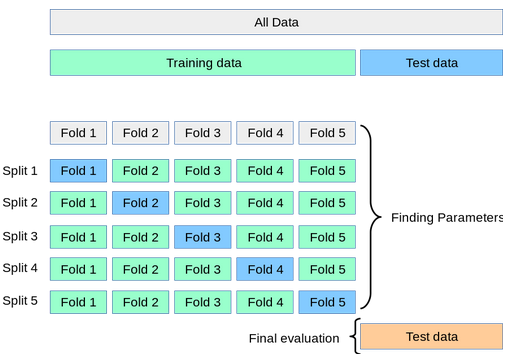
\includegraphics[width=0.75\textwidth]{0.png}
    \caption{k-Fold Cross Validation Method, source: \href{https://scikit-learn.org/stable/modules/cross_validation.html}{\textcolor{blue}{\underline{scikit-learn.org}}}}
    \label{fig:1}
\end{figure}

\paragraph*{}The \textit{k}-Fold Cross Validation method is a better way to
evaluate model performance. It is more robust to the choice of training and
validation sets, and is more computationally efficient than the simple
method. The \textit{k}-Fold Cross Validation method involves splitting the
available data into \textit{k} equal sized subsets. Then for each \textit{i}
between 0 and \textit{k}-1, the model is trained on all subsets except the
\textit{ith} subset, and evaluated on the \textit{ith} subset. The average
performance of the model across all \textit{k} iterations is reported as the
model accuracy. 

\paragraph*{}The intended use of this method is to evaluate the difference in
model performance as hyperparemeters are varied, in order to choose the optimal
hyperperameters for the context, without leaking information from the validation set.
In this method, the final test data set is only consulted after the hyperparameters
have been chosen. The implementation used in this assignment is shown below.

\begin{verbatim}
def kfold_cv(X, y, k, model):
  # Split the data into k folds
  X_folds = np.array_split(X, k)
  y_folds = np.array_split(y, k)
  accuracies = []
  for i in range(k):
    # Create training and validation sets
    # Training sets contain every fold except the ith
    X_train = np.concatenate(X_folds[:i] + X_folds[i+1:])
    y_train = np.concatenate(y_folds[:i] + y_folds[i+1:])
    # Validation set is the ith fold
    X_validation = X_folds[i]
    y_validation = y_folds[i]
    # Train the model
    model.fit(X_train, y_train)
    # Evaluate the model
    accuracies.append(model.score(X_validation, y_validation))
  return 1 - np.average(np.array(accuracies))
\end{verbatim}

\paragraph*{}A small (and likely unrepresentative) experiment was conducted
to choose a value for \textit{k} to use in this assigmnent. A Logistic Regression
model, using the default parameters was trained on the Fashion-MNIST dataset
and scored against the test set; the score was computed using the \textit{k}-Fold
Cross Validation implementation above with \textit{k} ranging from 5 to 10.
The results of this experiment are shown in Figure \ref{fig:3}. Since there was
no siginficant difference in outcome between the values of \textit{k} tested,
the value of 5 was chosen for the remainder of the experiments to reduce runtime.

\begin{figure}[ht]
    \centering
    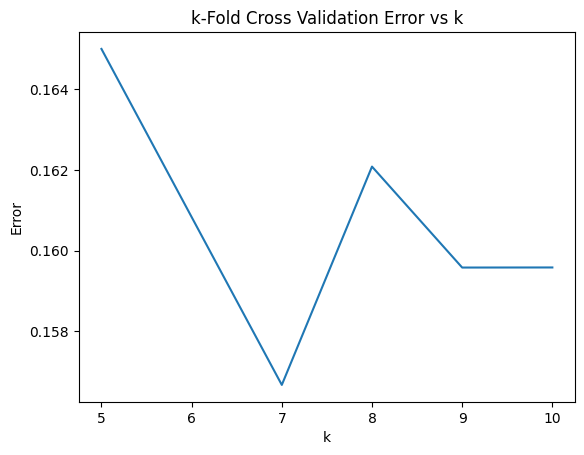
\includegraphics[width=0.75\textwidth]{1.png}
    \caption{LR Model Error vs. k}
    \label{fig:3}
\end{figure}

\section{Logistic Regression} is a method for predicting discrete-valued labels
based on input features which may or may not be discrete. In the case of this
assignment the input vectors as 28x28 grayscale images with pixel values normalized 
to the range [0, 1]. The output labels are binary. Logistic Regression is used
to learn (estimate) the underlying probability function which maps input vectors
to output label likelihoods. The probability function is estimated using the
maximum likelihood estimation.

\paragraph*{}Logistic Regression can be thought of as a neural network in which
the input features are multiplied by a weights matrix, the results are summed
together and offset by a bias parameter.
\begin{equation}
    z = \sum_{i=1}^{n} w_i x_i + b
\end{equation}
Logistic Regression introduces a nonlinearity after the linear unit in the
form of the sigmoid function to map the output of the linear model to the range
[0, 1]. The sigmoid function is defined as
\begin{equation}
    \sigma(z) = \frac{1}{1 + e^{-z}}
\end{equation}
In binary classification, the output of the sigmoid function is then interpreted
as the possibility thatthe input vector is an example of the positive class. The
complementary probability represents the likelihood of the input example
belonging to thenegative case.

In the first experiment, the effects of the regularization parameter \textit{C}
on the Logistic Regression model were investigated. The regularization parameter
is a hyperparameter which specifies the degree to which the model is penalized
for having large weights. In this experiment, higher values of \textit{C} correspond
to less regularization. The results of varying \textit{C} are shown in Figure
\ref{fig:4}, note that the x-axis is presented on a logarithmic scale.

\begin{figure}[ht]
    \centering
    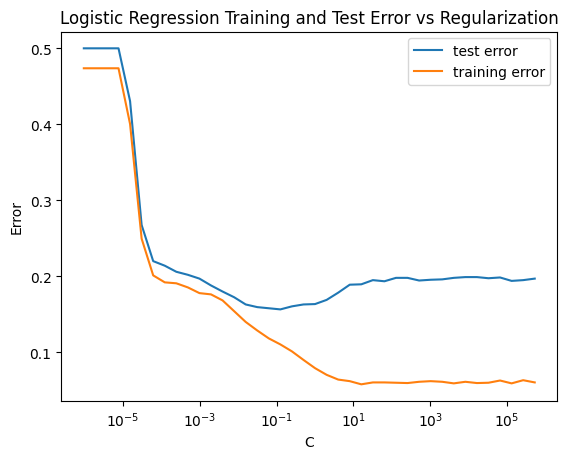
\includegraphics[width=0.75\textwidth]{2.png}
    \caption{LR Model Error vs. C}
    \label{fig:4}
\end{figure}

\paragraph*{}The results of this experiment show that the model performs best
when \textit{C} is set to approximately 10\^-1. High levels of regularization (the
left side of the plot) show that high model error indicating that the model is
underfitting the data as it is unable to learn the underlying probability function
due to the restriction. It appears to be underfitting as both the training
and testing error are quite high. On the right side of the plot, at much lower levels
of regularization the model appears to show a classic pattern of overfitting
where the training error continues to decrease while the testing error reaches
a minimum and then begins to increase with decreasing regularization.

\section{Support Vector Machines}

\paragraph*{}Support Vector Machines are a supervised learning method which can
be used in classification problems. The method attempts to find a hyperplane 
through the input space which seperates the data and categorizes them correctly.
The complexity of the hyperplane is controlled by the kernel used. In this experiment
a linear kernel was used. The hyperplane is found by maximizing the margin between
the hyperplane and the nearest data points on either side. During learning, a hyperplane
which minimizes training error is learned.

\paragraph*{}This experiment varied the regularization parameter \textit{C} in
the same way as the previous experiment. The results of this experiment are shown
in Figure \ref{fig:5}. The results show a similar pattern as the previous, with
high levels of regularization resulting in underfitting and low levels of regularization
resulting in overfitting. In both cases the model error is quite high.
The optimal value of \textit{C} appears to be approximately 10\^2.

\begin{figure}[ht]
    \centering
    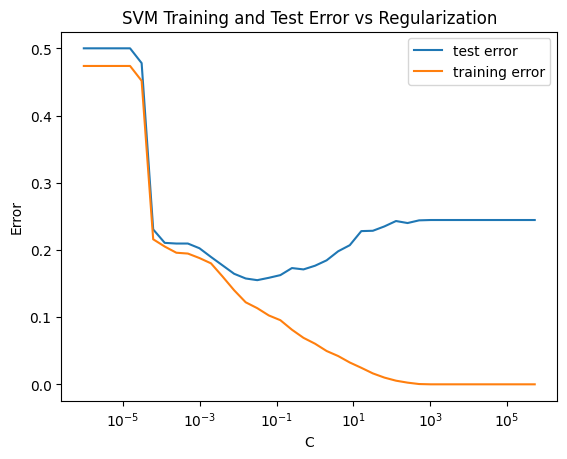
\includegraphics[width=0.75\textwidth]{3.png}
    \caption{SVM Model Error vs. C}
    \label{fig:5}
\end{figure}

\subsection{Finding the Optimal Regularization Parameter}

\paragraph*{}For both the Logistic Regression and Support Vector Machine models,
the regularization parameter \textit{C} was varied in the range [2\^-15, 2\^11].
This range was chosen at it fully encompased the range of values which produced
the best results in the previous experiments. Both classifiers were trained on 
the training set, and scored using k-fold cross validation. The purpose of this
section is to find the optimal value of \textit{C} for each model withtout 
involving the test set. This represents a hyperparameter search before 
the final model weights are learned; so that the model can better approximate
the true underlying distribution without overfitting to the test set.

\paragraph*{}The results of this experiment are shown in Figure \ref{fig:6}. The
bounds of the search as just wide enough to see the underfitting / overfitting
pattern from the previous experiments. Both models reach an optimal value near
the same point.

\begin{verbatim}
    Logistic Regression Minimum Error:      0.15083
    Optimal Logistic Regression C Value:    0.06250
    SVM Minimum Error:                      0.15291
    Optimal SVM C Value:                    0.03125
\end{verbatim}

\begin{figure}[ht]
    \centering
    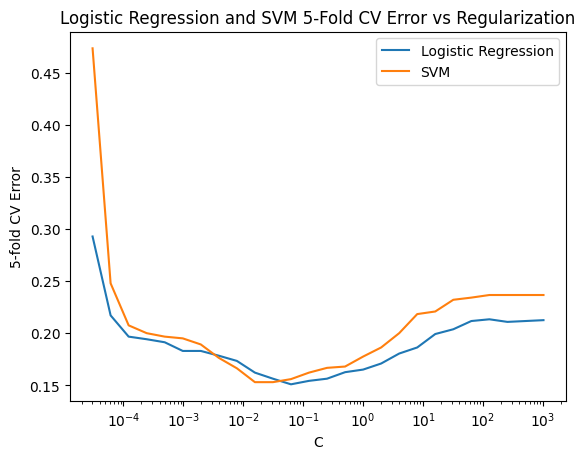
\includegraphics[width=0.75\textwidth]{4.png}
    \caption{Model Error vs. Regularization, Using 5-fold Cross Validation}
    \label{fig:6}
\end{figure}

\paragraph*{}The two models were compared by computing the difference in their
log loss scores on the test set. This calculation provides a more confident way
of determining the better performing model. The confidence value is calculated 
according to:
\begin{equation}
    \frac{1}{n} \sum_{i=1}^{n} [\ell (y_i, \hat{h}_1(x_i)) - \ell (y_i, \hat{h}_2(x_i))]
\end{equation}
where
\begin{equation}
    \ell(y, \hat{y}) = -ylog \hat{y} - (1-y) log (1-\hat{y})
\end{equation}
The resulting confidence values was 2.212, a decidedly positive value indicating
that the second hypothesis, in this case the SVM, is better than the first.

\section{Gaussian Kernel SVM}

\paragraph*{}The previous experiments used a linear kernel for the Support Vector
Machine model. In this experiment a Gaussian kernel was used. Gaussian SVM models
use a bandwidth paramter, $\gamma$ to control the sensitivity of the kernel to 
the distance to near data points. Higher values of $\gamma$ result in a more 
complicated decision surfaces which bend more radically to fit the data, and
therefore is also more prone to overfitting. To combat overfitting for a given
value of $\gamma$, the regularization parameter \textit{C} was varied for each $\gamma$
value tried. The result was to product a series of pairs, each containing a choice
for $\gamma$ and the correspondingly optimal choice for \textit{C}.

\paragraph*{}The results of this experiment are shown in Figure \ref{fig:7}. The
horizontal axis represents the bandwidth parameter $\gamma$, and ther vertical
represents the error of a model trained with the $\gamma$, \textit{C} pair.

\begin{verbatim}
        SVM Minimum Error:      0.14749
        SVM Gamma Value:        0.00781
        SVM C Value:            4.0
\end{verbatim}

\begin{figure}[ht]
    \centering
    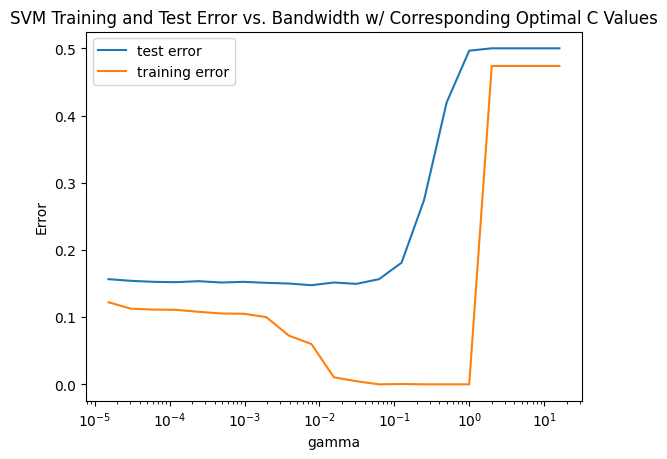
\includegraphics[width=0.75\textwidth]{5.png}
    \caption{Model Error vs. Bandwidth Parameter, Using 5-fold Cross Validation}
    \label{fig:7}
\end{figure}

\paragraph*{}The results of this experiment show that the model performs best
when $\gamma$ is set to approximately 0.0078, with a correspondingly high regularization
term of 4.0. Using a Gaussian kernel has improved the performance of the model;
reducing the error from 15.29\% to 14.75\%.

\end{document}